We conducted two different experiments, one to predict the force measured
by the force sensor and another one to classify the grasp type.
%The EMG data were preprocessed as described in Section \ref{sec:preproc}.

As already mentioned in Section \ref{sec:adapt}, our working
assumption is to have $N$ pre-trained models stored in memory; new
data comes from subject $N+1$ and the system starts training, to build
the $N+1$'th model. The performance is then evaluated using unseen
data from subject $N+1$. To simulate this scenario and to have a
reliable estimation of the performance, we use a leave-one-out
approach: out of the $10$ subjects for which we have data recordings,
we train $9$ models off-line; these correspond to the $N$ stored
models in memory, while data from the remaining subject are be used
for the adaptive learning of the $N+1$'th model. The training
sequences are random subsets from the entire dataset, that is taken
without considering the order in which they were acquired. This
procedure is repeated $10$ times, using in turn all the recorded
subjects for the adaptive learning of the model.

To assess the performance of the proposed adaptation method we
compared it to two baseline methods. The first one, that we call
\emph{Prior}, consists in using only the pre-trained models without
updating them with the new training data; then we consider only the
best performance of the $9$ pre-trained models, corresponding to the
best-case scenario. The second one, \emph{NoAdapt}, is plain LS-SVM
using only the new data for training, as it would be in the standard
scenario without adaption.

As a measure of performance, for classification we use the standard
classification rate; for regression, the performance index is the
correlation coefficient evaluated between the predicted force signal
and the real one. The choice of the correlation coefficient, as
opposed to the more standard Mean-Square Error, is suggested by a
practical consideration: when driving a prosthesis, or even a
non-prosthetic mechanical hand, we are not interested in the absolute
force values desired by the user/subject, since mechanical hands
usually cannot apply as much force as human hands do, for obvious
safety reasons\footnote{Or, e.g., in teleoperation scenarios, they
could be able to apply \emph{much more} force than a human hand
can.}. We are rather concerned about getting a signal which is
\emph{strongly correlated} with the user/subject's will. To build the
pre-trained models we used the standard SVM algorithm. All the
parameters to be set during training ($C$ and $\gamma$ of the gaussian
kernel) were chosen by cross-validation.

Figure \ref{fig:diff_cla} shows the average difference between the
classification performance of \emph{NoAdapt} and our method.
Adaptation always improves the performance, although the standard
deviation is rather large when training is done on too few samples:
depending on the subject, the improvement can be large (up to about
$11\%$) or small, and a slight loss in performance appears in the
worst cases. This is due to the high variance of the leave-one-out
error with few training samples. Still, the average gain is almost
$5\%$ when there are only $30$ training samples; and it settles to
around $1\%$ with smaller standard deviation, as the number of
training samples increase.

To get a more detailed idea, consider Figure \ref{fig:cla_abs}: panel
$(a)$ shows the performance obtained on the ``best'' subject, while
panel $(b)$ shows the worst. In the best case the gain is about
\textbf{FRA: mettici qualche numero!}, while in the worst case we
basically re-obtain the performance of \emph{NoAdapt}, as soon as
enough samples from the new distribution are considered.

This last case represents the paradigmatic case of no previous models
matching the distribution of the new subject; as a consequence, the
parameter $\beta$ was automatically set to a very small value. In this
case, there is essentially no transfer of prior knowledge. This shows
that, if we neglect the behaviour of the system when very few samples
have been considered, in the worst case the adaptation mechanism will
perform as well as the non-adapting case. Moreover, it is reasonable
to think that the overall performance of the method would increase
with the number of stored models, as this means a larger probability
of finding a matching pre-trained model. In the long run, a large,
possibly categorised, database of pre-trained models would definitely
help getting uniformly better performances.

Note that in all cases the performance of \emph{Prior} models are
well below the performance of \emph{Adapt} and \emph{NoAdapt}: in
Figure \ref{fig:cla_abs} we show only the performance of the best one
among the $9$ stored models. Similar observations can be done for the
regression task in Figure \ref{fig:diff_reg} and Figure
\ref{fig:reg_abs}. In particular we gain on average $5\%$ correlation
when the first $30$ samples are considered; then the gain seems to
decrease, approaching $0$ when enough new training samples are
acquired. However note that the standard deviation bars are all above
the zero, meaning that in worst case most of the time we do not lose
anything compared to the NoAdapt model (cf. Figure \ref{fig:reg_abs},
panel $(b)$).

\begin{figure}[t]
  \centering
  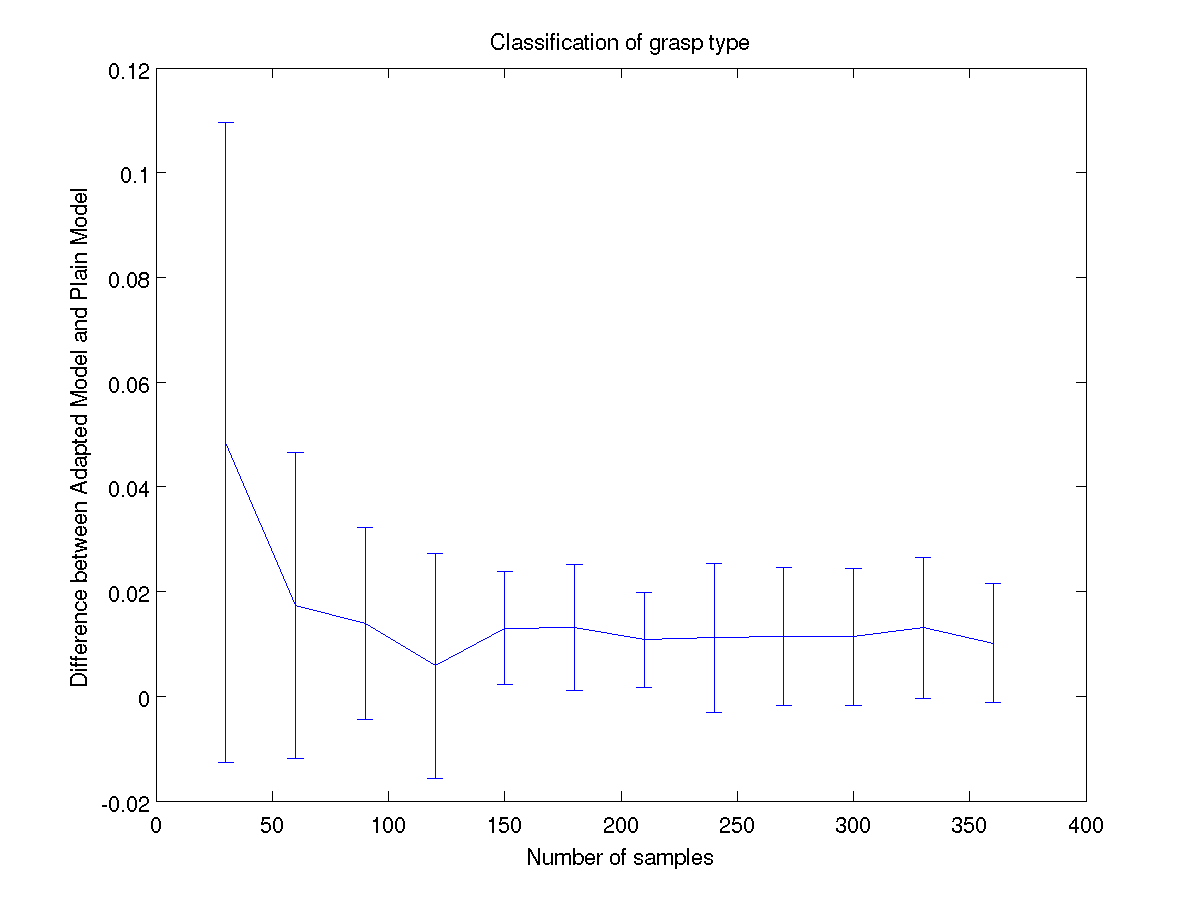
\includegraphics[width=0.95\linewidth]{figs/exp1}
  \caption{Classification: difference in performance between
    \emph{NoAdapt} and our method.}
  \label{fig:diff_cla}
\end{figure}

\begin{figure*}[ht] \centering
  \begin{tabular}{cc}
    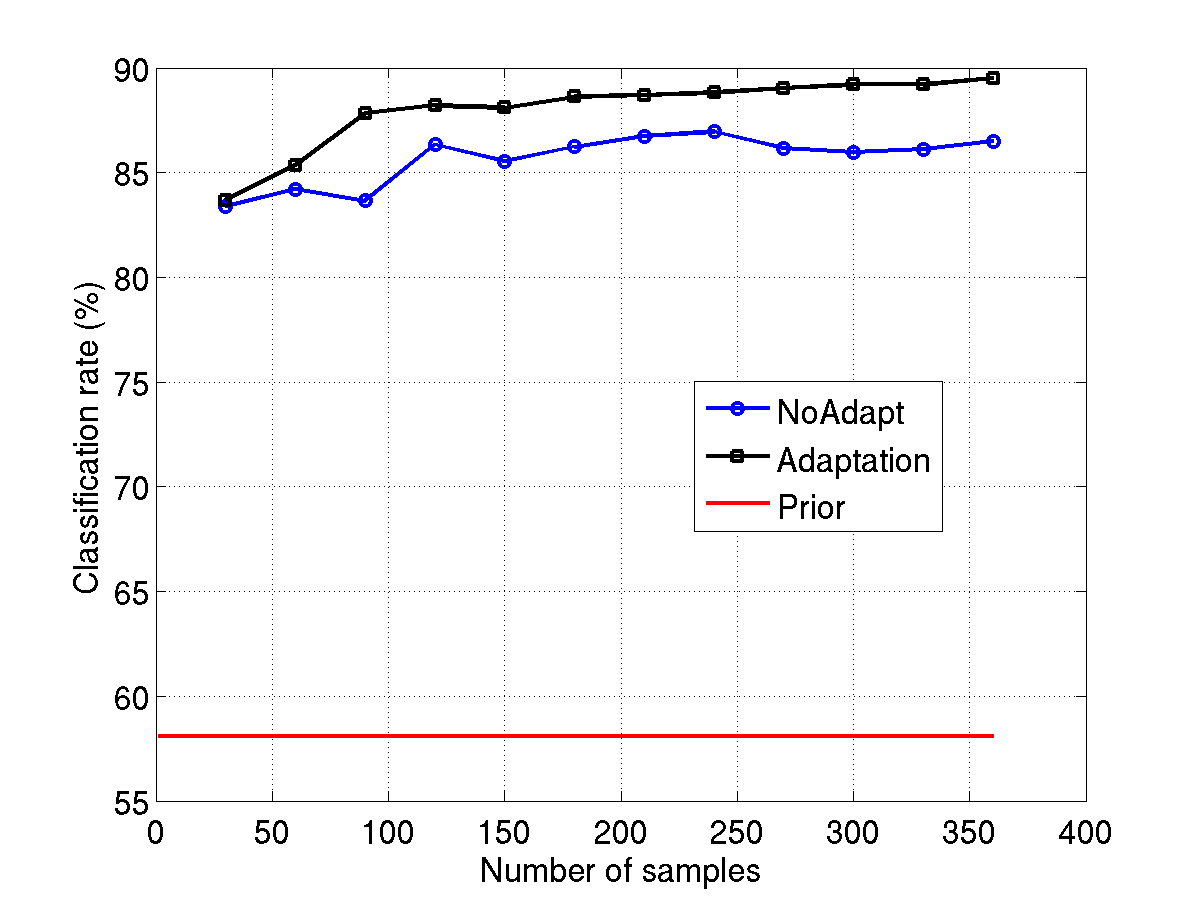
\includegraphics[width=0.45\textwidth]{figs/exp1_abs_best} &
    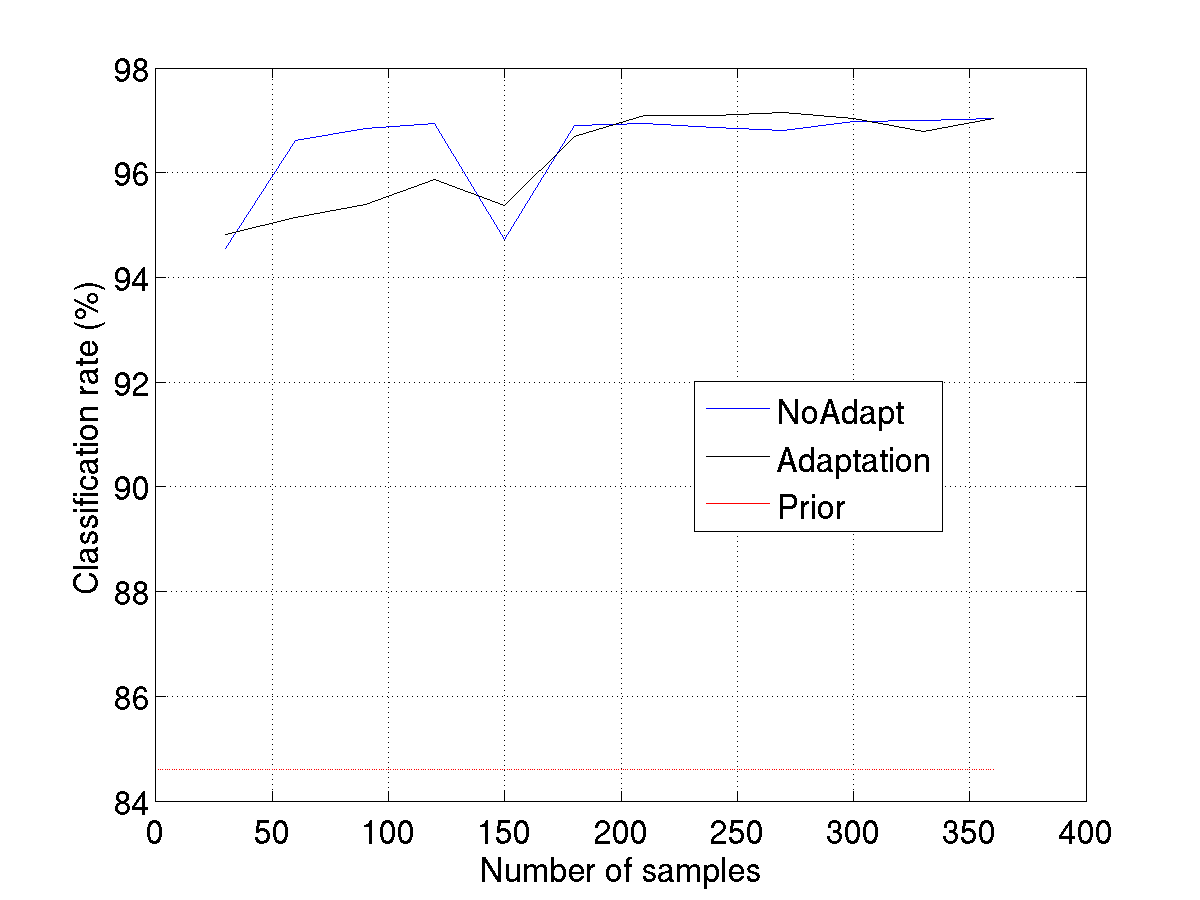
\includegraphics[width=0.45\textwidth]{figs/exp1_abs_worst} \\
    $(a)$ & $(b)$ \\
  \end{tabular}
  \caption{Classification: $(a)$ classification rate gain
    of the adapted model compared to \emph{NoAdapt} and \emph{Prior}
    on the best behaving subject; $(b)$ classification rate gain for
    the worst subject.}
  \label{fig:cla_abs}
\end{figure*}

\begin{figure}[ht]
  \centering
  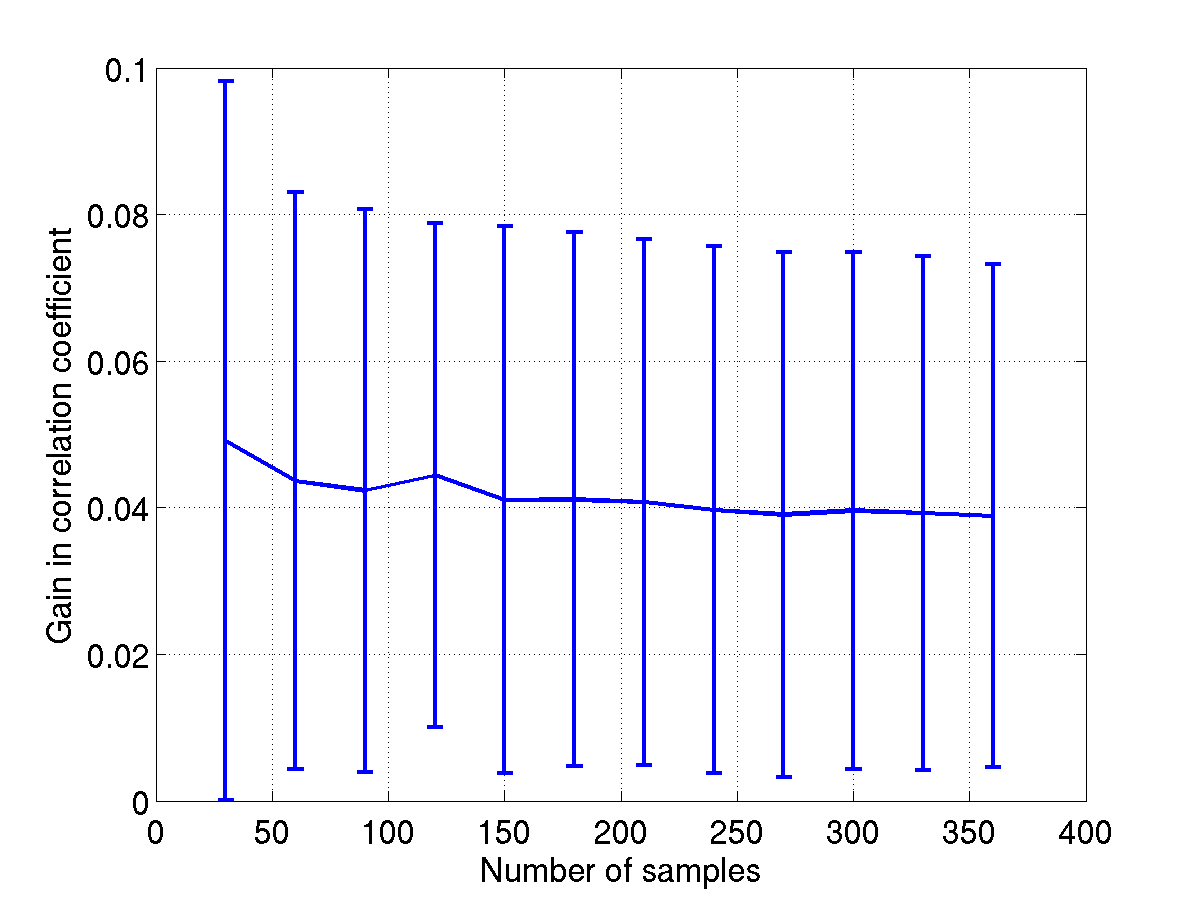
\includegraphics[width=0.95\linewidth]{figs/exp2}
  \caption{Regression: difference in performance between
    \emph{NoAdapt} and our method.}
  \label{fig:diff_reg}
\end{figure}

\begin{figure*}[ht] \centering
  \begin{tabular}{cc}
    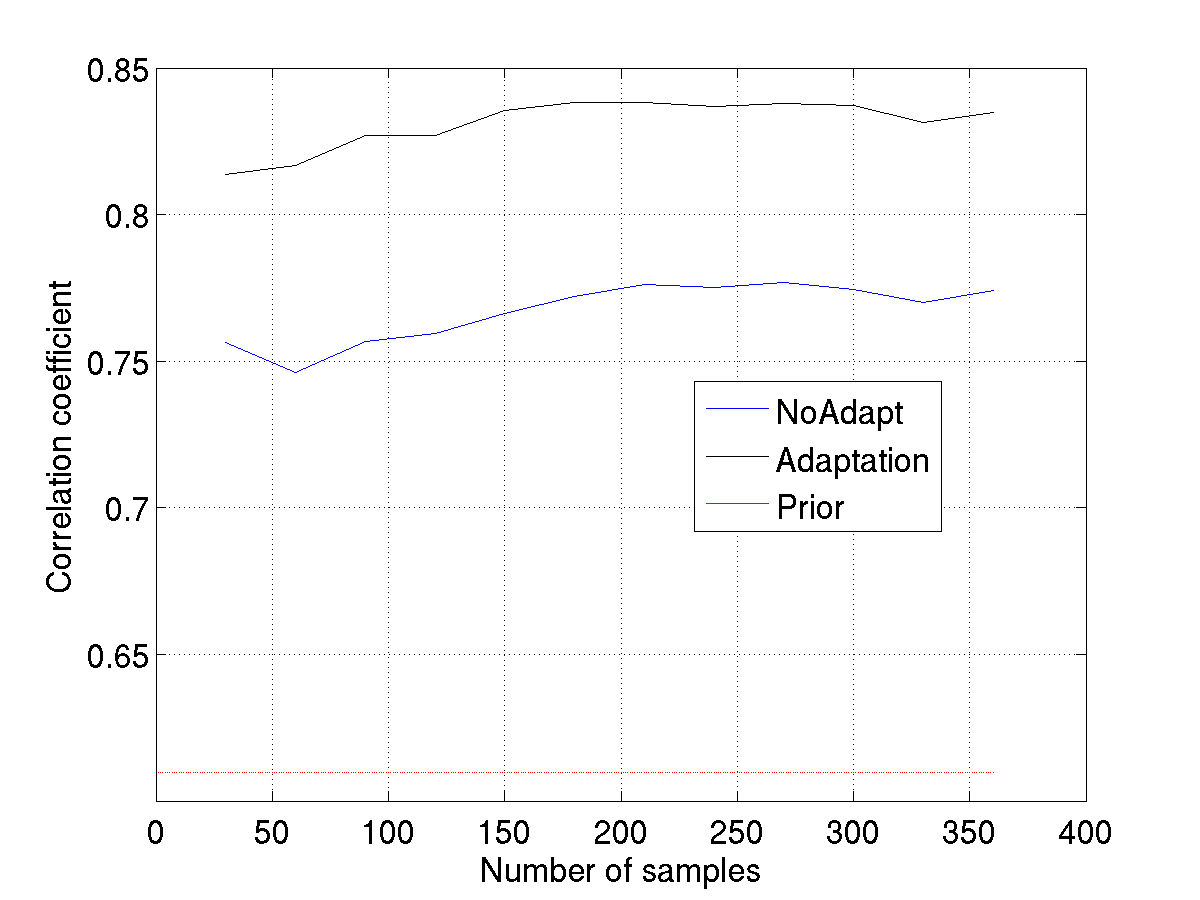
\includegraphics[width=0.45\textwidth]{figs/exp2_abs_best} &
    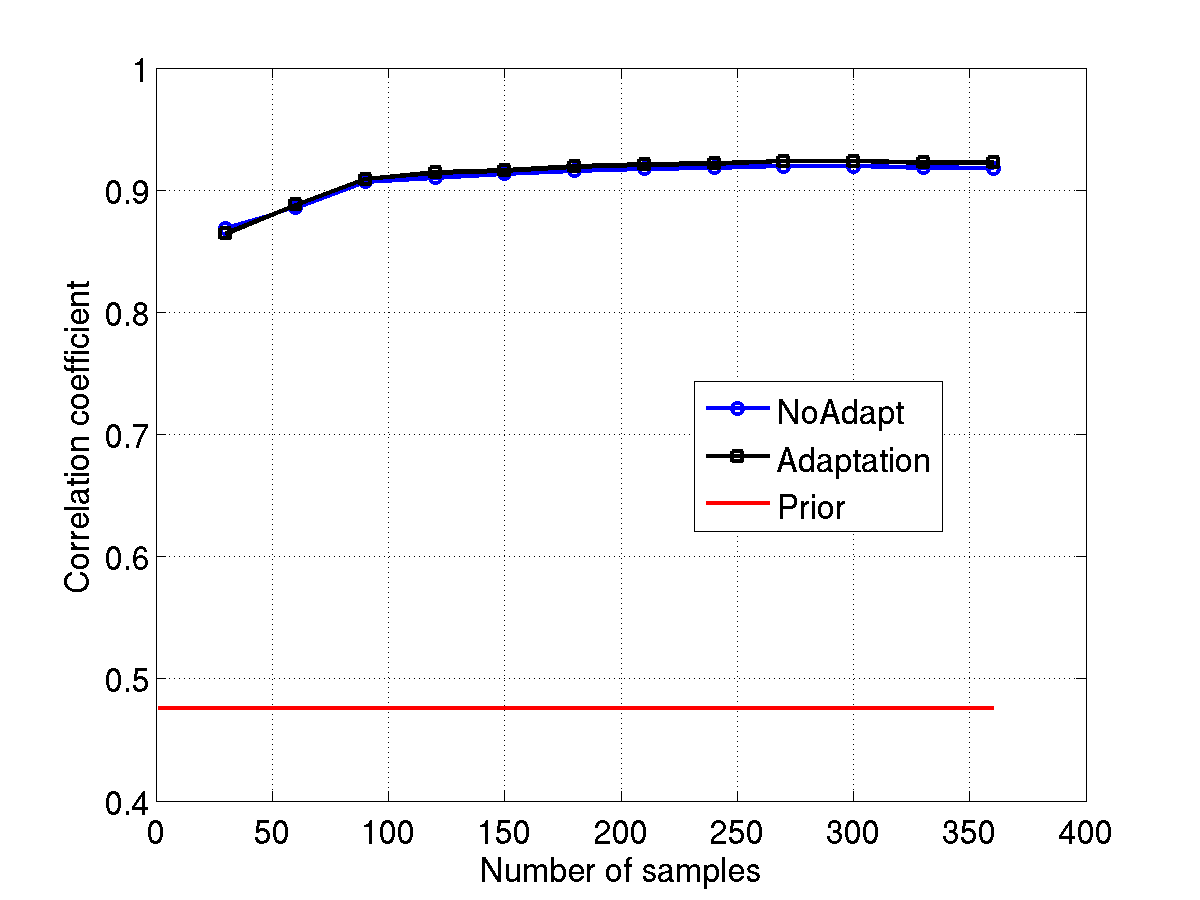
\includegraphics[width=0.45\textwidth]{figs/exp2_abs_worst} \\
    $(a)$ & $(b)$ \\
  \end{tabular}
  \caption{Regression: $(a)$ classification rate gain
    of the adapted model compared to \emph{NoAdapt} and \emph{Prior}
    on the best behaving subject; $(b)$ classification rate gain for
    the worst subject.}
  \label{fig:reg_abs}
\end{figure*}
